\section{Result 4: certifying the die-level false-alarm rate}
\label{sec:result-4}

A frozen stage-2 scorer gives every candidate a score, and a die is flagged at threshold $t$ iff
some candidate's score exceeds $t$. $p(t)$ is the probability that a defect-free die is flagged,
and $\hat p_m(t)$ the fraction of $m$ i.i.d.\ defect-free certification dies that are flagged.

\begin{theorem}[Result 4]
\label{thm:4}
For a grid $t_1<\dots<t_T$ fixed before the certification dies are drawn, with probability at
least $1-\delta$, simultaneously for all $j$,
\[ p(t_j)\le\hat p_m(t_j)+\sqrt{\frac{\ln(T/\delta)}{2m}}. \]
So the selected threshold $\hat t$, the lowest $t_j$ whose right-hand side is at most $\alpha$,
satisfies $p(\hat t)\le\alpha$ with probability at least $1-\delta$ (if no $t_j$ qualifies, nothing
is certified).
\end{theorem}

\begin{proof}
Fix $j$. The flags $X_i=\mathbb 1[\text{die }i\text{ flagged at }t_j]$ are independent
Bernoulli$(p(t_j))$, because the dies are i.i.d.\ and the scorer and grid are fixed. Hoeffding's
inequality \citep{hoeffding1963probability} for the $[0,1]$-valued variables $1-X_i$ gives
$\P\bigl(\frac1m\sum_i(1-X_i)-(1-p(t_j))\ge\epsilon\bigr)\le e^{-2m\epsilon^2}$, that is,
$\P(p(t_j)-\hat p_m(t_j)\ge\epsilon)\le e^{-2m\epsilon^2}$. By the union bound over the $T$ grid points,
$\P(\exists j:p(t_j)-\hat p_m(t_j)\ge\epsilon)\le Te^{-2m\epsilon^2}$, which equals $\delta$ at
$\epsilon=\sqrt{\ln(T/\delta)/(2m)}$. On the complementary event every $t_j$ obeys the inequality,
in particular the data-dependent $\hat t$, whose right-hand side is $\le\alpha$ by construction.
\end{proof}

\begin{inshort}
\begin{enumerate}[leftmargin=*]
  \item Each threshold's false-alarm count is a sum of i.i.d.\ coin flips: one-sided Hoeffding,
    $e^{-2m\epsilon^2}$.
  \item The threshold is chosen from the data, so protect all $T$ at once: union bound,
    $Te^{-2m\epsilon^2}=\delta$. Choosing costs $\ln T$ under the square root.
  \item The grid must be fixed before the certification dies are seen (here: from the validation pool).
\end{enumerate}
\end{inshort}

\paragraph{Measured vs.\ theory (E4).} Overlapping regime; $\alpha=\EFourAlpha$, $\delta=0.05$,
$T=\EFourT$. Fixed before any certification die is drawn: the scorer (norm-constrained logistic
regression on the hand-crafted features, trained once on $\EFourNTrain$ candidates, $B=\EFourScorerB$
by validation, validation error $\EFourScorerValError$) and the grid (quantiles of the validation
pool's nuisance scores). Each of $R=\EFourRepeats$ repeats uses fresh defect-free dies. The true
false-alarm rate is the flag frequency on the far-test pool ($\EFourNFar$ dies). The check fixed
before running, a violation fraction $\le\delta$ at every $m$, holds.

\begin{center}
\small
\begin{tabular}{rccccc}
\toprule
$m$ & margin $\sqrt{\ln(T/\delta)/2m}$ & certifiable & certified bound & true FAR & defective dies flagged \\
\midrule
500 & $\EFourFiveHundredMargin$ & \EFourFiveHundredCert & $\EFourFiveHundredCertBound$ & $\EFourFiveHundredTrueFar$ & $\EFourFiveHundredDetect$ \\
1{,}000 & $\EFourOneKMargin$ & \EFourOneKCert & $\EFourOneKCertBound$ & $\EFourOneKTrueFar$ & $\EFourOneKDetect$ \\
2{,}000 & $\EFourTwoKMargin$ & \EFourTwoKCert & $\EFourTwoKCertBound$ & $\EFourTwoKTrueFar$ & $\EFourTwoKDetect$ \\
4{,}000 & $\EFourFourKMargin$ & \EFourFourKCert & $\EFourFourKCertBound$ & $\EFourFourKTrueFar$ & $\EFourFourKDetect$ \\
8{,}000 & $\EFourEightKMargin$ & \EFourEightKCert & $\EFourEightKCertBound$ & $\EFourEightKTrueFar$ & $\EFourEightKDetect$ \\
\bottomrule
\end{tabular}

{\small Certified bound, true FAR and detection are means over the repeats that certified.}
\end{center}

No repeat selected a threshold whose true rate exceeds $\alpha$ (largest: $\EFourMaxSelectedFar$).
Given the scorer, grid and far-test pool, the repeats' violation indicators are i.i.d.\
Bernoulli$(q)$, and zero violations have probability $(1-q)^R\le e^{-qR}<\delta$ whenever
$q>\ln(1/\delta)/R$; so with confidence $1-\delta$ the violation rate is at most
$\ln(1/\delta)/R=\EFourViolBoundZero$, below $\delta$ as the theorem says.

Nothing can be certified below $m=\EFourMinMPossible$, where the margin alone exceeds $\alpha$;
$m=\EFourSmallestM$ certifies in every repeat. Since the rule leaves room for the margin, the
selected thresholds land far below $\alpha$, and more dies buy sensitivity: detection
$\EFourTwoKDetect$ at $m=2{,}000$ and $\EFourEightKDetect$ at $m=8{,}000$, against $\EFourOracleDetect$
for the threshold one would pick knowing $p(t)$.

\begin{figure}[tb]
  \centering
  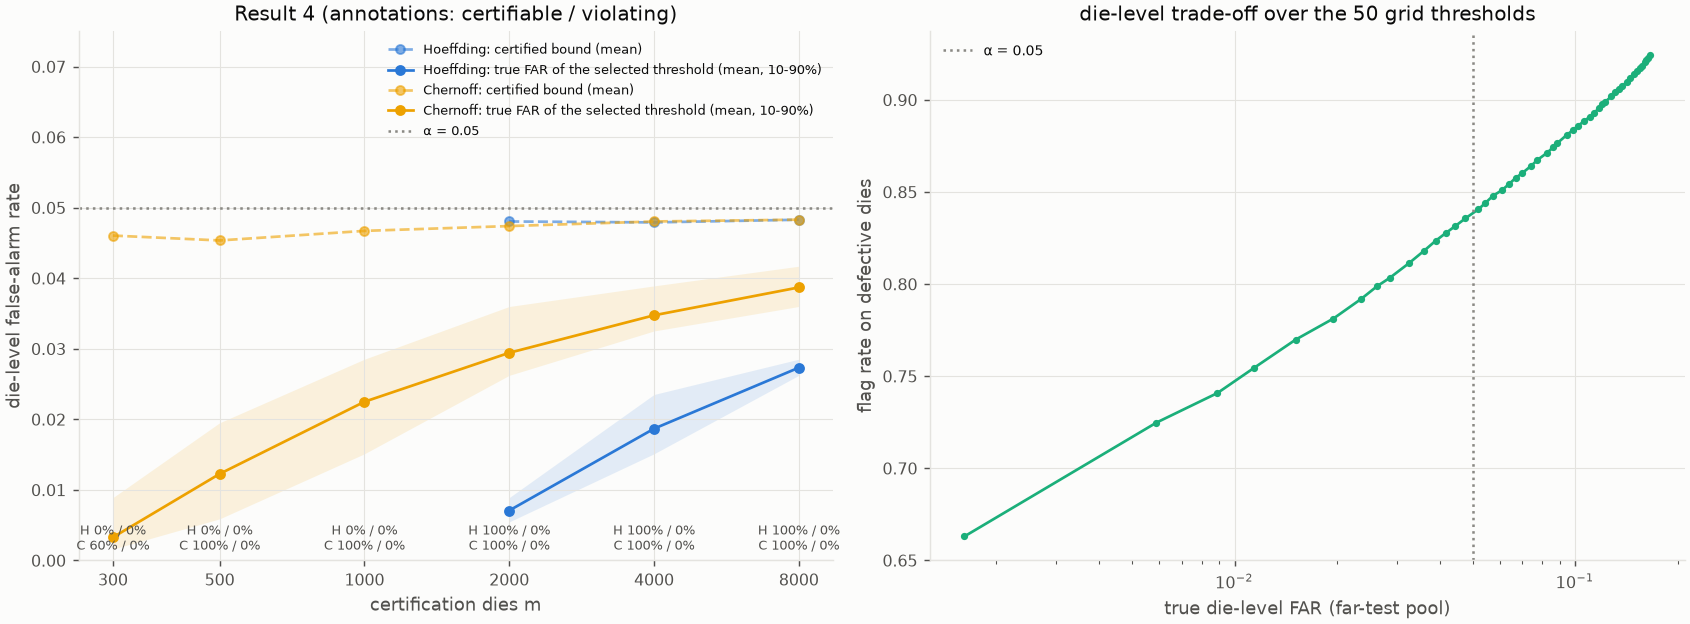
\includegraphics[width=0.8\linewidth]{../figures/e4_false_alarms.png}
  \caption{E4: certified bound and true false-alarm rate of the selected threshold vs.\ $m$
  (left; annotations: fraction of repeats that certified and that violated), and the die-level
  trade-off over the grid (right).}
  \label{fig:e4}
\end{figure}
